\documentclass[conference]{IEEEtran}
\IEEEoverridecommandlockouts
% The preceding line is only needed to identify funding in the first footnote. If that is unneeded, please comment it out.
\usepackage{cite}
\usepackage{amsmath,amssymb,amsfonts}
\usepackage{algorithmic}
\usepackage{graphicx}
\usepackage{textcomp}
\usepackage{xcolor}

\usepackage[hyphenbreaks]{breakurl}
\usepackage[hyphens]{url}

% spanish symbols for narrative
\usepackage[utf8]{inputenc} 
% language
\usepackage[spanish]{babel} 

%changing from roman number to integers
\renewcommand{\thesection}{\arabic{section}}
\renewcommand{\thesubsection}{\arabic{section}.\arabic{subsection}} 

%\renewcommand\topfraction{.9}
%\renewcommand\textfraction{0.35}
%\renewcommand\floatpagefraction{0.8}

\usepackage{pgfplots}
\usepackage{pgfplotstable}
    \pgfplotsset{
        % use this `compat' level or higher to position the bars in one group
        % next to each other
        compat=1.7,
    }
    % load the data table ...
    \pgfplotstableread[col sep=comma]{misc/dtFemaleAgeDistribution.csv}{\femaleAgeDistribution}
        % and store the number of columns in `\NoOfCols'
        % (minus 1 because counting in `\foreach' starts with zero
        \pgfplotstablegetcolsof{\femaleAgeDistribution}
        \pgfmathtruncatemacro{\NoOfCols}{\pgfplotsretval-1}

%packages used for models diagrams
\usepackage{tikz}
\usetikzlibrary{babel}
\usetikzlibrary{shapes.geometric}
\usetikzlibrary{arrows.meta,arrows}
\usepackage[T1]{fontenc}
\usepackage{textcomp}
\usepackage[left=2cm,right=2cm]{geometry}
\usepackage{graphicx}
\usepackage{amsmath}
\usepackage{pifont}
\usepackage{adjustbox}

\def\BibTeX{{\rm B\kern-.05em{\sc i\kern-.025em b}\kern-.08em
    T\kern-.1667em\lower.7ex\hbox{E}\kern-.125emX}}
\begin{document}
\title{Título\\
}

\author{\IEEEauthorblockN{Autores}
\IEEEauthorblockA{
\textit{Grupo de Investigación de Aprendizaje Profundo} \\
\textit{Departamento Ingeniería en Sistemas de Información}\\
\textit{Universidad Tecnológica Nacional}\\
\textit{Facultad Regional Rosario}\\
mail@frro.utn.edu.ar} %should be hyperlink
}

\maketitle

%\renewcommand{\abstractname}{Abstract} %Ajustes por traducción a español
%\begin{abstract}
%
%This document is a model and instructions for \LaTeX.
%This and the IEEEtran.cls file define the components of your paper [title, text, heads, etc.]. *CRITICAL: Do Not Use Symbols, Special Characters, Footnotes, or Math in Paper Title or Abstract.
%\end{abstract}

%\renewcommand{\IEEEkeywordsname}{Palabras Clave} %Ajustes por traducción a español
%\begin{IEEEkeywords}
%aprendizaje profundo, red neuronal convolucional, rsna, procesamiento de imagenes
%\end{IEEEkeywords}

\section*{Abstract}

\textit
{
La evaluación de la edad ósea esquelética es una práctica clínica comúnmente utilizada para investigar la madurez del sistema esquelético de un niño. Esta práctica puede ayudar a los médicos a diagnosticar afecciones que retrasan o aceleran el crecimiento y desarrollo físico. Recientemente, el advenimiento y la proliferación de redes neuronales convolucionales (RNC) ha mostrado ser prometedor en una variedad de aplicaciones de imágenes médicas. En este documento proponemos y probamos varios enfoques de aprendizaje profundo para evaluar la madurez ósea de forma automática comparando dos enfoques: por un lado, una RNC general que estima madurez ósea sobre radiografías de género masculino y femenino; por el otro, dos RNC especializadas cada una en su género respectivo. \textbf{Los resultados mostraron que la utilización de un/dos modelo/s general/especializado resulta más precisa para la estimación de madurez ósea.} Esta es una de las primeras evaluaciones automatizadas de la edad ósea esquelética probada en un conjunto de datos públicos donde se evalúa la utilización de una RNC general y dos RNC específicas para el género de la persona, para los cuales el código fuente está disponible, representando así una base exhaustiva para futuras investigaciones en el campo.
}

\section{Introducción}

Durante el desarrollo del organismo de una persona, los huesos del esqueleto cambian de tamaño y forma, los cuales responden a una determinada edad ósea. Diferencia entre la edad ósea estimada de un niño y su edad cronológica podría indicar trastornos del crecimiento y anomalías endocrinas \cite{AproachToSkeletalMaturation}. Los médicos utilizan la evaluación de la edad ósea para estimar la madurez del sistema esquelético de un niño. Los métodos de evaluación de la edad ósea generalmente comienzan con tomar una sola imagen de rayos X de la mano izquierda desde la muñeca hasta las puntas de los dedos, ver Figura~\ref{fig:mano}. Los huesos en la imagen de rayos X se comparan con radiografías en un atlas estandarizado de desarrollo óseo. Tal atlas de edad ósea se basa en un gran número de radiografías recogidas de niños del mismo sexo y edad.

\begin{figure}[ht!]
  \centering
  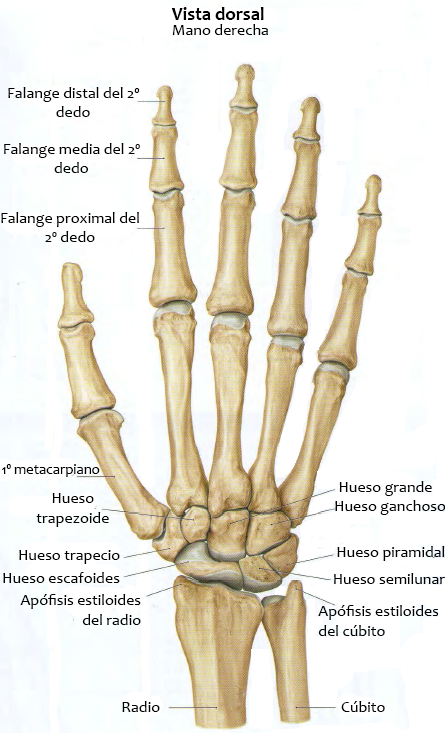
\includegraphics[scale=0.7]{misc/imgHuesosMano.png}
  \caption{Huesos de una mano y muñeca humana adaptada de \cite{AtlasMedicina}}
  \label{fig:mano}
\end{figure}

En las últimas décadas, el procedimiento de evaluación de la edad ósea se realizó de forma manual utilizando los métodos de Greulich y Pyle (GP) \cite{GP} o de Tanner-Whitehouse (TW) \cite{TW3}. El procedimiento GP determina la edad ósea al comparar la radiografía del paciente con un atlas de edades representativas. La técnica TW se basa en un sistema de puntuación que examina 20 huesos específicos. En ambos casos, el procedimiento de evaluación ósea requiere un tiempo considerable; a su vez, la precisión en la estimación depende de la experiencia del radiólogo y tiende a ser subjetiva. 

Desde 1992, preocupaciones sobre la variabilidad interobservador en la estimación manual de la edad ósea \cite{GP_variability} han llevado al establecimiento de varios métodos automáticos computarizados para la estimación de la misma. Los recientes avances en el aprendizaje profundo y sus aplicaciones a la visión por computadora permitieron a muchos investigadores mejorar drásticamente los resultados obtenidos con los sistemas de procesamiento de imágenes particularmente relacionados con el análisis de imágenes médicas \cite{DeepLearningInBiology}. A diferencia de las técnicas tradicionales de aprendizaje automático, las técnicas de aprendizaje profundo permiten que un algoritmo se programe a sí mismo aprendiendo de las imágenes dadas a un gran conjunto de datos de ejemplos etiquetados, eliminando así la necesidad de especificar reglas \cite{DeepLearning}. Los enfoques basados en aprendizaje profundo están ganando más atención porque en varios casos se demostró que logran e incluso superan el rendimiento a nivel humano, lo que hace que el procesamiento de imágenes de extremo a extremo sea automatizado y suficientemente rápido. En el campo de las imágenes médicas, las redes neuronales convolucionales (RNC) se han utilizado con éxito para el cribado de retinopatía diabética \cite{DeepLearningInDiabetics}, diagnóstico de enfermedades cardíacas \cite{DeepLearningInHeartDiseases}, detección de cáncer de pulmón \cite{DeepLearningLungCancer} y otras aplicaciones \cite{DeepLearningInBiology}. En el caso de la evaluación de la edad ósea, el mismo es un procedimiento que realizado manualmente requiere alrededor de 30 minutos de tiempo del médico por cada paciente. Cuando se realiza el mismo procedimiento utilizando un software basado en los métodos clásicos de visión por computadora, toma de 1 a 5 minutos, pero aún requiere una considerable supervisión y experiencia médica. Los métodos basados en aprendizaje profundo permiten evitar la ingeniería de características al aprender automáticamente la jerarquía de características discriminatorias directamente de un conjunto de ejemplos etiquetados. Usando un enfoque de aprendizaje profundo, el procesamiento de una imagen generalmente toma menos de 1 segundo, mientras que la precisión de estos métodos en muchos casos excede la de los métodos convencionales. Soluciones de redes neuronales profundas para la evaluación de la edad ósea de radiografías de mano han sido sugeridas \cite{DeepLearningAssesingSkeletalMaturity1,DeepLearningAssesingSkeletalMaturity2,DeepLearningAssesingSkeletalMaturity3}. Sin embargo, ninguno de estos ha evaluado en profundidad la conveniencia de separar el conjunto de datos de acuerdo al género de la radiografía y generar una RNC por cada género para investigar la precisión resultante de los mismos. 

En este trabajo se investiga si una RNC especializada en un determinado género podría ser más precisa en estimar la edad de una persona de acuerdo a la radiografía de su mano en lugar de una que utilice radiografías de ambos géneros. Nuestra contribución consiste en explorar el comportamiento de una RNC de acuerdo al conjunto de datos que es ingresado en la misma. Validamos la precisión de estas redes neuronales utilizando los datos de el desafío pediátrico de edad ósea 2017 organizado por la Sociedad Radiológica de América del Norte (RSNA) \cite{RSNAChallenge}. Este conjunto de datos ahora está disponible de manera gratuita y puede ser accedido en \cite{RSNADataSet}.

\section{Metodología y Objetivos}

\subsection{Conjunto de datos}

The IEEEtran class file is used to format your paper and style the text. All margins, 
column widths, line spaces, and text fonts are prescribed; please do not 
alter them. You may note peculiarities. For example, the head margin
measures proportionately more than is customary. This measurement 
and others are deliberate, using specifications that anticipate your paper 
as one part of the entire proceedings, and not as an independent document. 
Please do not revise any of the current designations.

% used PGFPlots v1.14

\begin{tikzpicture}
    \begin{semilogyaxis}[
        % adjust the `width' a bit by keeping the default `height'
        width=1.05*\axisdefaultwidth,
        height=\axisdefaultheight,
        % set appropriate `ymax' value so the `nodes near coords' fit to the plot
        % (adjusting the `ymin' value is just to make it look a little bit better)
        ymin=0,
        ymax=2000,
        % there should be no gap between the bars in one group
        ybar=0pt,
        % use data from the table for the xticklabels
        xtick=data,
        xticklabels from table={\femaleAgeDistribution}{Anio},
        % adjust the size of the bars so they don't overlap
        % (you can play with the numerator to change the gap between the groups)
        bar width=0.6/\NoOfCols,
        % enlarge the x limits so all of the bars are shown
        % (play with the value to adjust the gap on the sides of the plot)
        enlarge x limits={abs=0.6},
        % and position the legend outside of the plot to not overlap with the data
        %legend pos=outer north east,
        % add `nodes near coords'
        nodes near coords={
            % because internally PGFPlots works with floating point numbers, we
            % change them to fixed point numbers
            \pgfkeys{
                /pgf/fpu=true,
                /pgf/fpu/output format=fixed,
            }
            % truncate value count to integer
            \pgfmathparse{\pgfplotspointmeta}
            \pgfmathprintnumber{\pgfmathresult}\,
        },
        % set the style of the `nodes near coords'
        nodes near coords style={
            font=\tiny,
            rotate=90,
            anchor=west,
        },
        % as basis for the `nodes near coords' use the raw y values
        point meta=rawy,
        ymin=1,
    ]
        % add the data rows for each column 
        \foreach \i in {1,...,\NoOfCols} {
            \addplot table [
                x expr=\coordindex,
                y index=\i,
                col sep=comma,
            ] {\femaleAgeDistribution};
                % to automatically add the legend entries first extract the
                % column name and store it in `\colname'
                    \pgfplotstablegetcolumnnamebyindex{\i}\of{\femaleAgeDistribution}\to{\colname}
                % now you can add the legend entry
                % (because we are in a loop we have to use the "expanded" version)
                \addlegendentryexpanded{\colname};
        }
    \end{semilogyaxis}
\end{tikzpicture}


\subsection{Preprocesamiento}
Define abbreviations and acronyms the first time they are used in the text, 
even after they have been defined in the abstract. Abbreviations such as 
IEEE, SI, MKS, CGS, ac, dc, and rms do not have to be defined. Do not use 
abbreviations in the title or heads unless they are unavoidable.

\subsection{Modelos}

\begin{center}
\begin{adjustbox}{width=\columnwidth}
	\begin{tikzpicture}[scale = 1]	
		\node[inner sep=0pt] (russell) at (-0.6,1.8)
    {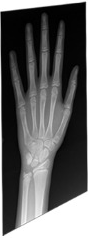
\includegraphics[scale=0.65]{misc/imgRadiografia.png}};
		%FLECHA
		\node[inner sep=0pt] (russell) at (0.55,1.95)
    {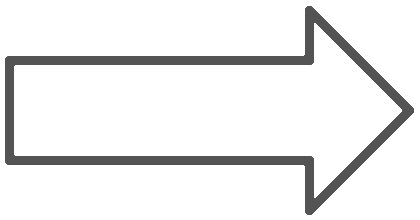
\includegraphics[scale=0.06]{misc/imgArrowOutline.png}};
		%PRIMER CUBO
		\draw[thick,-](1.5,1,1)--(1.5,3,1);
		\draw[thick,-](1.5,3,1)--(1.75,3,1);
		\draw[thick,-](1.75,3,1)--(1.75,1,1);
		\draw[thick,-](1.75,1,1)--(1.5,1,1);
		\draw[thick,-](1.5,3,1)--(1.5,3,-1);		
		\draw[thick,-](1.5,3,-1)--(1.75,3,-1);
		\draw[thick,-](1.75,3,-1)--(1.75,3,1);
		\draw[thick,-](1.75,3,-1)--(1.75,1,-1);
		\draw[thick,-](1.75,1,-1)--(1.75,1,1);
		%SEGUNDO RECTANGULO
		\draw[thick,-](4,1.5,1)--(4,2.5,1);
		\draw[thick,-](4,2.5,1)--(4,2.5,0);
		\draw[thick,-](4,2.5,0)--(4,1.5,0);
		\draw[thick,-](4,1.5,0)--(4,1.5,1);
		%UNIONES ENTRE 1° Y 2° FIGURA
		\draw[thick,dashed,-](1.75,3,1)--(4,2.5,1);
		\draw[thick,dashed,-](1.75,1,1)--(4,1.5,1);
		\draw[thick,dashed,-](1.75,3,-1)--(4,2.5,0);
		\draw[thick,dashed,-](1.75,1,-1)--(4,1.5,0);
		%FLECHA
		\draw[thick,->](4.6,2.3,1)--(5.75,2.3,1);
		%TERCER RECTANGULO 
		\draw[thick,-](6,1.25,1)--(6,3.25,1);
		\draw[thick,-](6,3.25,1)--(6.25,3.25,1);
		\draw[thick,-](6.25,3.25,1)--(6.25,1.25,1);
		\draw[thick,-](6.25,1.25,1)--(6,1.25,1);
		%FLECHA
		\draw[thick,->](6.35,2.3,1)--(7.9,2.3,1);
		%CUARTO RECTANGULO 
		\draw[thick,-](8,1.25,1)--(8,3.25,1);
		\draw[thick,-](8,3.25,1)--(8.25,3.25,1);
		\draw[thick,-](8.25,3.25,1)--(8.25,1.25,1);
		\draw[thick,-](8.25,1.25,1)--(8,1.25,1);
		%FLECHA
		\draw[thick,->](8.35,2.3,1)--(9.125,2.3,1);
		%QUINTO RECTANGULO 
		\draw[thick,-](9.225,1.25,1)--(9.225,3.25,1);
		\draw[thick,-](9.225,3.25,1)--(9.475,3.25,1);
		\draw[thick,-](9.475,3.25,1)--(9.475,1.25,1);
		\draw[thick,-](9.475,1.25,1)--(9.225,1.25,1);
		%FLECHA
		\draw[thick,->](9.575,2.3,1)--(10.25,2.3,1);
		%SEXTO RECTANGULO 
		\draw[thick,-](10.35,1.25,1)--(10.35,3.25,1);
		\draw[thick,-](10.35,3.25,1)--(10.60,3.25,1);
		\draw[thick,-](10.60,3.25,1)--(10.60,1.25,1);
		\draw[thick,-](10.60,1.25,1)--(10.35,1.25,1);
		%FLECHA
		\draw[thick,->](10.7,2.3,1)--(11.375,2.3,1);
		%SEPTIMO RECTANGULO 
		\draw[thick,-](11.475,1.25,1)--(11.475,3.25,1);
		\draw[thick,-](11.475,3.25,1)--(11.725,3.25,1);
		\draw[thick,-](11.725,3.25,1)--(11.725,1.25,1);
		\draw[thick,-](11.725,1.25,1)--(11.475,1.25,1);
		%FLECHA
		\draw[thick,->](11.825,2.3,1)--(12.5,2.3,1);
		%OCTAVO RECTANGULO 
		\draw[thick,-](12.6,1.5,1)--(12.6,3,1);
		\draw[thick,-](12.6,3,1)--(12.85,3,1);
		\draw[thick,-](12.85,3,1)--(12.85,1.5,1);
		\draw[thick,-](12.85,1.5,1)--(12.6,1.5,1);
		%FLECHA
		\draw[thick,->](12.95,2.3,1)--(13.625,2.3,1);
		%NOVENO RECTANGULO 
		\draw[thick,-](13.725,1.5,1)--(13.725,3,1);
		\draw[thick,-](13.725,3,1)--(13.975,3,1);
		\draw[thick,-](13.975,3,1)--(13.975,1.5,1);
		\draw[thick,-](13.975,1.5,1)--(13.725,1.5,1);
		%FLECHA
		\draw[thick,->](14.075,2.3,1)--(14.9,2.3,1);
		%DECIMO RECTANGULO 
		\draw[thick,-](15,1.7,1)--(15,2.8,1);
		\draw[thick,-](15,2.8,1)--(15.25,2.8,1);
		\draw[thick,-](15.25,2.8,1)--(15.25,1.7,1);
		\draw[thick,-](15.25,1.7,1)--(15,1.7,1);
		%FLECHA HACERLA DOBLE
		\node[inner sep=0pt] (russell) at (15.25,1.88)
    {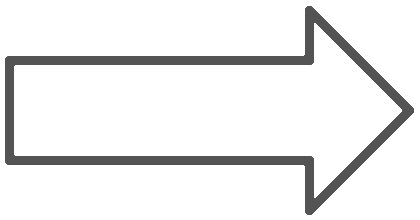
\includegraphics[scale=0.04]{misc/imgArrowOutline.png}};
		%ONCEAVO RECTANGULO 
		\draw[thick,-](16,1.9,1)--(16,2.6,1);
		\draw[thick,-](16,2.6,1)--(18,2.6,1);
		\draw[thick,-](18,2.6,1)--(18,1.9,1);
		\draw[thick,-](18,1.9,1)--(16,1.9,1);
		%TEXTOS
		\node[scale=0.65] at (16.625,1.98) {Y};
		\node[scale=0.65] at (16.625,1.7) {edad ósea estimada};
		\node[scale=1] at (5.75,0.68) {\ding{115}};
		\node[scale=0.75] at (5.7,0.35) {salida rn50 1000};
		\node[scale=1] at (7.75,0.68) {\ding{115}};
		\node[scale=0.75] at (7.8,0.35) {densa 1000 relu};
		\node[scale=1] at (8.95,3.1) {\ding{116}};
		\node[scale=0.75] at (8.95,3.4) {dropout 0,2};
		\node[scale=1] at (10.1,0.68) {\ding{115}};
		\node[scale=0.75] at (10.1,0.35) {densa 1000 relu};
		\node[scale=1] at (11.22,3.1) {\ding{116}};
		\node[scale=0.75] at (11.25,3.4) {dropout 0,2};
		\node[scale=1] at (12.35,0.9) {\ding{115}};
		\node[scale=0.75] at (12.4,0.6) {densa 240 relu};
		\node[scale=1] at (13.457,2.8) {\ding{116}};
		\node[scale=0.75] at (13.4,3.1) {dropout 0,1};
		\node[scale=1] at (14.75,1.1) {\ding{115}};
		\node[scale=0.75] at (14.9,0.8) {densa 1 regresión};
		\node[scale=1] at (4.2,3.2) {ResNet-50};
		\node[scale=1.4] at (3.5,4.5) {Convolución};
		\node[scale=1.4] at (11,4.5) {Capas totalmente conectadas};
		\node[inner sep=0pt] (russell) at (3.35,3.75)
    {
\includegraphics[width=4.5cm,height=0.25cm]{misc/imgLlave.png}};
		\node[inner sep=0pt] (russell) at (10.6,3.75)
    {
\includegraphics[width=10cm,height=0.25cm]{misc/imgLlave.png}};
	\end{tikzpicture}
\end{adjustbox}
\end{center}


\begin{center}
\begin{adjustbox}{width=\columnwidth}
	\begin{tikzpicture}[scale = 1]	
		\node[inner sep=0pt] (russell) at (-0.6,3.05)
    {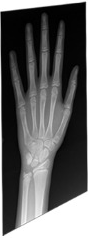
\includegraphics[scale=0.65]{misc/imgRadiografia.png}};
		%FLECHA
		\node[inner sep=0pt] (russell) at (0.55,3.2)
    {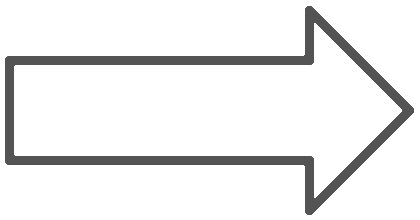
\includegraphics[scale=0.06]{misc/imgArrowOutline.png}};
		%PRIMER CUBO
		\draw[thick,-](1.5,2.25,1)--(1.5,4.25,1);
		\draw[thick,-](1.5,4.25,1)--(1.75,4.25,1);
		\draw[thick,-](1.75,4.25,1)--(1.75,2.25,1);
		\draw[thick,-](1.75,2.25,1)--(1.5,2.25,1);
		\draw[thick,-](1.5,4.25,1)--(1.5,4.25,-1);		
		\draw[thick,-](1.5,4.25,-1)--(1.75,4.25,-1);
		\draw[thick,-](1.75,4.25,-1)--(1.75,4.25,1);
		\draw[thick,-](1.75,4.25,-1)--(1.75,2.25,-1);
		\draw[thick,-](1.75,2.25,-1)--(1.75,2.25,1);
		%SEGUNDO RECTANGULO
		\draw[thick,-](4,2.75,1)--(4,3.75,1);
		\draw[thick,-](4,3.75,1)--(4,3.75,0);
		\draw[thick,-](4,3.75,0)--(4,2.75,0);
		\draw[thick,-](4,2.75,0)--(4,2.75,1);
		%UNIONES ENTRE 1° Y 2° FIGURA
		\draw[thick,dashed,-](1.75,4.25,1)--(4,3.75,1);
		\draw[thick,dashed,-](1.75,2.25,1)--(4,2.75,1);
		\draw[thick,dashed,-](1.75,4.25,-1)--(4,3.75,0);
		\draw[thick,dashed,-](1.75,2.25,-1)--(4,2.75,0);
		%FLECHA
		\draw[thick,->](4.6,3.55,1)--(5.75,3.55,1);
		%TERCER RECTANGULO 
		\draw[thick,-](6,2.5,1)--(6,4.5,1);
		\draw[thick,-](6,4.5,1)--(6.25,4.5,1);
		\draw[thick,-](6.25,4.5,1)--(6.25,2.5,1);
		\draw[thick,-](6.25,2.5,1)--(6,2.5,1);
		%FLECHA
		\draw[thick,->](6.35,3.55,1)--(7.6,2.3,1);
		%CUADRADO inferior
		\draw[thick,-](2.55,-0.75,1)--(2.55,1.25,1);
		\draw[thick,-](2.55,1.25,1)--(4.55,1.25,1);
		\draw[thick,-](4.55,1.25,1)--(4.55,-0.75,1);
		\draw[thick,-](4.55,-0.75,1)--(2.55,-0.75,1);
		%FLECHA inferior
		\node[inner sep=0pt] (russell) at (4.85,-0.1)
    {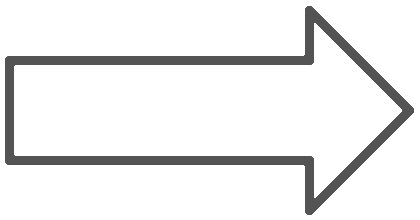
\includegraphics[scale=0.06]{misc/imgArrowOutline.png}};
		%RECTANGULO inferior
		\draw[thick,-](5.85,-0.25,1)--(5.85,0.75,1);
		\draw[thick,-](5.85,0.75,1)--(6.1,0.75,1);
		\draw[thick,-](6.1,0.755,1)--(6.1,-0.25,1);
		\draw[thick,-](6.1,-0.25,1)--(5.85,-0.25,1);
		%FLECHA diagonal desde inferior a superior
		\draw[thick,->](6.2,0.25,1)--(7.6,2.1,1);
		%CUARTO RECTANGULO 
		\draw[thick,-](7.7,1.25,1)--(7.7,3.25,1);
		\draw[thick,-](7.7,3.25,1)--(7.95,3.25,1);
		\draw[thick,-](7.95,3.25,1)--(7.95,1.25,1);
		\draw[thick,-](7.95,1.25,1)--(7.7,1.25,1);
		%FLECHA
		\draw[thick,->](8.05,2.3,1)--(8.65,2.3,1);
		%QUINTO RECTANGULO 
		\draw[thick,-](8.75,1.25,1)--(8.75,3.25,1);
		\draw[thick,-](8.75,3.25,1)--(9,3.25,1);
		\draw[thick,-](9,3.25,1)--(9,1.25,1);
		\draw[thick,-](9,1.25,1)--(8.75,1.25,1);
		%FLECHA
		\draw[thick,->](9.1,2.3,1)--(9.7,2.3,1);
		%SEXTO RECTANGULO 
		\draw[thick,-](9.8,1.25,1)--(9.8,3.25,1);
		\draw[thick,-](9.8,3.25,1)--(10.05,3.25,1);
		\draw[thick,-](10.05,3.25,1)--(10.05,1.25,1);
		\draw[thick,-](10.05,1.25,1)--(9.8,1.25,1);
		%FLECHA
		\draw[thick,->](10.15,2.3,1)--(10.75,2.3,1);
		%SEXTO RECTANGULO 
		\draw[thick,-](10.85,1.25,1)--(10.85,3.25,1);
		\draw[thick,-](10.85,3.25,1)--(11.1,3.25,1);
		\draw[thick,-](11.1,3.25,1)--(11.1,1.25,1);
		\draw[thick,-](11.1,1.25,1)--(10.85,1.25,1);
		%FLECHA
		\draw[thick,->](11.2,2.3,1)--(11.8,2.3,1);
		%SEPTIMO RECTANGULO 
		\draw[thick,-](11.9,1.25,1)--(11.9,3.25,1);
		\draw[thick,-](11.9,3.25,1)--(12.15,3.25,1);
		\draw[thick,-](12.15,3.25,1)--(12.15,1.25,1);
		\draw[thick,-](12.15,1.25,1)--(11.9,1.25,1);
		%FLECHA
		\draw[thick,->](12.25,2.3,1)--(12.85,2.3,1);
		%OCTAVO RECTANGULO 
		\draw[thick,-](12.95,1.5,1)--(12.95,3,1);
		\draw[thick,-](12.95,3,1)--(13.2,3,1);
		\draw[thick,-](13.2,3,1)--(13.2,1.5,1);
		\draw[thick,-](13.2,1.5,1)--(12.95,1.5,1);
		%FLECHA
		\draw[thick,->](13.30,2.3,1)--(13.85,2.3,1);
		%NOVENO RECTANGULO 
		\draw[thick,-](14,1.5,1)--(14,3,1);
		\draw[thick,-](14,3,1)--(14.25,3,1);
		\draw[thick,-](14.25,3,1)--(14.25,1.5,1);
		\draw[thick,-](14.25,1.5,1)--(14,1.5,1);
		%FLECHA
		\draw[thick,->](14.35,2.3,1)--(14.9,2.3,1);
		%DECIMO RECTANGULO 
		\draw[thick,-](15,1.7,1)--(15,2.8,1);
		\draw[thick,-](15,2.8,1)--(15.25,2.8,1);
		\draw[thick,-](15.25,2.8,1)--(15.25,1.7,1);
		\draw[thick,-](15.25,1.7,1)--(15,1.7,1);
		%FLECHA HACERLA DOBLE
		\node[inner sep=0pt] (russell) at (15.25,1.88)
    {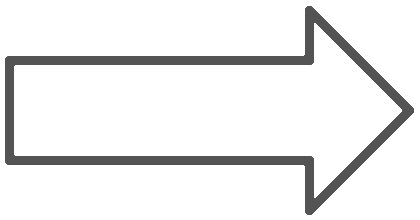
\includegraphics[scale=0.04]{misc/imgArrowOutline.png}};
		%ONCEAVO RECTANGULO 
		\draw[thick,-](16,1.9,1)--(16,2.6,1);
		\draw[thick,-](16,2.6,1)--(18,2.6,1);
		\draw[thick,-](18,2.6,1)--(18,1.9,1);
		\draw[thick,-](18,1.9,1)--(16,1.9,1);
		%TEXTOS
		\node[scale=0.65] at (16.625,1.98) {Y};
		\node[scale=0.65] at (16.625,1.7) {edad ósea estimada};
		\node[scale=1.4] at (3.2,0.25) {Género};
		\node[scale=1.4] at (3.2,-0.5) {M/F};
		\node[scale=1] at (5.6,-0.85) {\ding{115}};
		\node[scale=0.75] at (5.6,-1.15) {densa 32 relu};
		\node[scale=1] at (5.75,1.93) {\ding{115}};
		\node[scale=0.75] at (5.5,1.6) {salida rn50 1000};
		\node[scale=1] at (7.43,3.1) {\ding{116}};
		\node[scale=0.75] at (7.55,3.4) {concat 1032};
		\node[scale=1] at (8.5,0.68) {\ding{115}};
		\node[scale=0.75] at (8.5,0.35) {densa 1000 relu};
		\node[scale=1] at (9.53,3.1) {\ding{116}};
		\node[scale=0.75] at (9.53,3.4) {dropout 0,2};
		\node[scale=1] at (10.6,0.68) {\ding{115}};
		\node[scale=0.75] at (10.6,0.35) {densa 1000 relu};
		\node[scale=1] at (11.63,3.1) {\ding{116}};
		\node[scale=0.75] at (11.63,3.4) {dropout 0,2};
		\node[scale=1] at (12.7,0.9) {\ding{115}};
		\node[scale=0.75] at (12.7,0.6) {densa 240 relu};
		\node[scale=1] at (13.73,2.8) {\ding{116}};
		\node[scale=0.75] at (13.73,3.1) {dropout 0,1};
		\node[scale=1] at (14.75,1.1) {\ding{115}};
		\node[scale=0.75] at (14.9,0.8) {densa 1 regresión};
		\node[scale=1] at (4.2,4.45) {ResNet-50};
		\node[scale=1.4] at (3.5,5.75) {Convolución};
		\node[scale=1.4] at (11,5.75) {Capas totalmente conectadas};
		\node[inner sep=0pt] (russell) at (3.35,5)
    {
\includegraphics[width=4.5cm,height=0.25cm]{misc/imgLlave.png}};
		\node[inner sep=0pt] (russell) at (10.6,5)
    {
\includegraphics[width=10cm,height=0.25cm]{misc/imgLlave.png}};
	\end{tikzpicture}
\end{adjustbox}
\end{center}
\begin{itemize}
\item Use either SI (MKS) or CGS as primary units. (SI units are encouraged.) English units may be used as secondary units (in parentheses). An exception would be the use of English units as identifiers in trade, such as ``3.5-inch disk drive''.
\item Avoid combining SI and CGS units, such as current in amperes and magnetic field in oersteds. This often leads to confusion because equations do not balance dimensionally. If you must use mixed units, clearly state the units for each quantity that you use in an equation.
\item Do not mix complete spellings and abbreviations of units: ``Wb/m\textsuperscript{2}'' or ``webers per square meter'', not ``webers/m\textsuperscript{2}''. Spell out units when they appear in text: ``. . . a few henries'', not ``. . . a few H''.
\item Use a zero before decimal points: ``0.25'', not ``.25''. Use ``cm\textsuperscript{3}'', not ``cc''.)
\end{itemize}

\section{Resultados del experimento}
Number equations consecutively. To make your 
equations more compact, you may use the solidus (~/~), the exp function, or 
appropriate exponents. Italicize Roman symbols for quantities and variables, 
but not Greek symbols. Use a long dash rather than a hyphen for a minus 
sign. Punctuate equations with commas or periods when they are part of a 
sentence, as in:
\begin{equation}
a+b=\gamma\label{eq}
\end{equation}

Be sure that the 
symbols in your equation have been defined before or immediately following 
the equation. Use ``\eqref{eq}'', not ``Eq.~\eqref{eq}'' or ``equation \eqref{eq}'', except at 
the beginning of a sentence: ``Equation \eqref{eq} is . . .''

\section{Conclusiones y Trabajo Futuro}

Please use ``soft'' (e.g., \verb|\eqref{Eq}|) cross references instead
of ``hard'' references (e.g., \verb|(1)|). That will make it possible
to combine sections, add equations, or change the order of figures or
citations without having to go through the file line by line.

Please don't use the \verb|{eqnarray}| equation environment. Use
\verb|{align}| or \verb|{IEEEeqnarray}| instead. The \verb|{eqnarray}|
environment leaves unsightly spaces around relation symbols.

Please note that the \verb|{subequations}| environment in {\LaTeX}
will increment the main equation counter even when there are no
equation numbers displayed. If you forget that, you might write an
article in which the equation numbers skip from (17) to (20), causing
the copy editors to wonder if you've discovered a new method of
counting.

{\BibTeX} does not work by magic. It doesn't get the bibliographic
data from thin air but from .bib files. If you use {\BibTeX} to produce a
bibliography you must send the .bib files. 

{\LaTeX} can't read your mind. If you assign the same label to a
subsubsection and a table, you might find that Table I has been cross
referenced as Table IV-B3. 

{\LaTeX} does not have precognitive abilities. If you put a
\verb|\label| command before the command that updates the counter it's
supposed to be using, the label will pick up the last counter to be
cross referenced instead. In particular, a \verb|\label| command
should not go before the caption of a figure or a table.

Do not use \verb|\nonumber| inside the \verb|{array}| environment. It
will not stop equation numbers inside \verb|{array}| (there won't be
any anyway) and it might stop a wanted equation number in the
surrounding equation.

\subsection{Conclusiones}
\begin{itemize}
\item The word ``data'' is plural, not singular.
\item The subscript for the permeability of vacuum $\mu_{0}$, and other common scientific constants, is zero with subscript formatting, not a lowercase letter ``o''.
\item In American English, commas, semicolons, periods, question and exclamation marks are located within quotation marks only when a complete thought or name is cited, such as a title or full quotation. When quotation marks are used, instead of a bold or italic typeface, to highlight a word or phrase, punctuation should appear outside of the quotation marks. A parenthetical phrase or statement at the end of a sentence is punctuated outside of the closing parenthesis (like this). (A parenthetical sentence is punctuated within the parentheses.)
\item A graph within a graph is an ``inset'', not an ``insert''. The word alternatively is preferred to the word ``alternately'' (unless you really mean something that alternates).
\item Do not use the word ``essentially'' to mean ``approximately'' or ``effectively''.
\item In your paper title, if the words ``that uses'' can accurately replace the word ``using'', capitalize the ``u''; if not, keep using lower-cased.
\item Be aware of the different meanings of the homophones ``affect'' and ``effect'', ``complement'' and ``compliment'', ``discreet'' and ``discrete'', ``principal'' and ``principle''.
\item Do not confuse ``imply'' and ``infer''.
\item The prefix ``non'' is not a word; it should be joined to the word it modifies, usually without a hyphen.
\item There is no period after the ``et'' in the Latin abbreviation ``et al.''.
\item The abbreviation ``i.e.'' means ``that is'', and the abbreviation ``e.g.'' means ``for example''.
\end{itemize}


\subsection{Trabajo Futuro}
\textbf{The class file is designed for, but not limited to, six authors.} A 
minimum of one author is required for all conference articles. Author names 
should be listed starting from left to right and then moving down to the 
next line. This is the author sequence that will be used in future citations 
and by indexing services. Names should not be listed in columns nor group by 
affiliation. Please keep your affiliations as succinct as possible (for 
example, do not differentiate among departments of the same organization).


\begin{thebibliography}{00}
\bibitem{AproachToSkeletalMaturation} 
Zerin JM, Hernandez RJ. 
\textit{Approach to skeletal maturation}. 
Hand Clin 1991; 7:53–62

\bibitem{GP} 
Greulich, W.W., Pyle, S.I.
\textit{Radiographic atlas of skeletal development of the hand and wrist}. 
The American Journal of the Medical Sciences 238(3), 393, 1959

\bibitem{TW3} 
Tanner JM, Healy MJ, Goldstein H, Cameron N.
\textit{Assessment of skeletal maturity and prediction of adult height (TW3 method), 3rd ed}. 
London, UK: Saunders Company, 2001

\bibitem{GP_variability} 
Berst MJ, Dolan L, Bogdanowicz MM, Stevens MA, Chow S, Brandser EA.
\textit{Effect of knowledge of chronologic age on the variability of pediatric bone age determined using the Greulich and Pyle standards}. 
AJR 2001; 176:507–510

\bibitem{DeepLearningInBiology} 
Ching, T., Himmelstein, D.S., Beaulieu-Jones, B.K., Kalinin, A.A., Do, B.T., Way, G.P., Ferrero, E., Agapow, P.M., Xie, W., Rosen, G.L., et al.
\textit{Opportunities and obstacles for deep learning in biology and medicine}.
bioRxiv p. 142760 (2017)

\bibitem{DeepLearning} 
LeCun Y, Bengio Y, Hinton G.
\textit{Deep learning}.
Nature 2015; 521:436–444

\bibitem{DeepLearningInDiabetics}
Rakhlin, A.
\textit{Diabetic retinopathy detection through integration of deep learning classification framework}.
bioRxiv p. 225508 (2017)

\bibitem{DeepLearningInHeartDiseases}
Korshunova, I.
\textit{Diagnosing heart diseases with deep neural networks}.
\\\texttt{\url{https://irakorshunova.github.io/2016/03/15/heart.html}} (2016), online; accedido 29 de Julio de 2017


\bibitem{DeepLearningLungCancer}
Daniel Hammack and Julian de Wit.
\textit{2017 Data Science Bowl, Predicting Lung Cancer: 2nd place solution write-up}.
\\\texttt{\url{http://blog.kaggle.com/2017/06/29/2017-data-science-bowl-predicting-lung-cancer-2nd-place-solution-write-up-daniel-hammack-and-julian-de-wit/}} (2017), online; accedido 29 de Julio de 2017

\bibitem{DeepLearningAssesingSkeletalMaturity1}
Larson, D.B., Chen, M.C., Lungren, M.P., Halabi, S.S., Stence, N.V., Langlotz, C.P.
\textit{Performance of a deep-learning neural network model in assessing skeletal maturity on pediatric hand radiographs}.
Radiology p. 170236 (2017)

\bibitem{DeepLearningAssesingSkeletalMaturity2}
Lee, H., Tajmir, S., Lee, J., Zissen, M., Yeshiwas, B.A., Alkasab, T.K., Choy, G., Do, S.
\textit{Fully automated deep learning system for bone age assessment}.
Journal of Digital Imaging pp. 1–15 (2017)

\bibitem{DeepLearningAssesingSkeletalMaturity3}
Spampinato, C., Palazzo, S., Giordano, D., Aldinucci, M., Leonardi, R.
\textit{Deep learning for automated skeletal bone age assessment in X-ray images}.
Medical image analysis 36, 41–51 (2017)

\bibitem{RSNAChallenge}
\textit{RSNA Pediatric Bone Age Challenge}.
\\\texttt{\url{http://rsnachallenges.cloudapp.net/competitions/4}} (2017), online; accedido 29 de julio de 2017

\bibitem{RSNADataSet}
Stanford University Artificial Intelligence in Medicine \& Imaging
\textit{Bone age images used in the 2017 RSNA bone age challenge competition}.
\\\texttt{\url{https://aimi.stanford.edu/available-labeled-medical-datasets}} 
(2017), online; accedido 29 de julio de 2017


\bibitem{AtlasMedicina}
Gilroy, A.M., MacPherson B.R., Ross L.M., Schünke M., Schulte E., Schumacher U., Voll M., Wesker K.
\textit{Prometheus. Atlas de Anatomía}.
pp 298, 2008
\end{thebibliography}




\end{document}
